\chapter{Optimization on manifolds} \label{chap:manifolds}

\epigraphhead[79]{
\epigraph{I am continuously amazed at how delightfully illuminating
differential geometry is.  If everyone listened to it then we would have so
many fewer janky algorithms out there. Until then <goes back to LaTeX'ing>...}{
\(\mathfrak{Michael ``El Muy Muy''
Betancourt}\)~\citep{betanalphaDiffGeometry}}
}

Despite hyperbolic neural networks as promoted by Ganea and B\'ecigneul are
ultimately built in terms of Ungar's gyrovector formalism coming from Physics,
and motivating arguments rather refer  to works in hyperbolic geometry, the
unifying language that does allow to connect the pieces and then formulate
computational algorithms is that of Differential Geometry. The goal of this appendix
is to give a feeling of what language we would like to see being used in the field.
We introduce some of the basic notions -- ones that can be introduced in short time
without much sacrifice -- and provide the links and directions as to where to search
for details.
We'll also be touching upon the Geoopt package and perspectives for improving
it.

In this thesis, we try to follow the language and approach demonstrated in
Frederic Schuller's lectures~\cite{geometricAnatomy,gravityLight}, as it seems
consistent enough and at the same time elucidating (and more rigorous than that
of e.g.~\citep{leeSmooth,leeRiem}). Rather than just reading this appendix, it
may be worth to acquaint with that course. We allow ourselves small abuses of
notation, such as using the same partial derivative symbol \( \partial_i \) for
functions acting on different instances of \( \mathbb{R}^n \).

\section{Differential geometry trivia}

We start with recalling, that an \( n \)-dimensional \emph{topological
manifold} is a ``nice'' topological space \( (M, \theta) \) that ``locally
looks like \(\mathbb{R}^n\)''.  The ``looks like'' translates as ``homeomorphic
to'', since topology is the only structure we've mentioned so far.
Specifically, each point \( p\in M \) has a neighbourhood \( U\subset M \) and
a homeomorphism (continuous map with continuous inverse) \( x:U \to
x(U)\subset\mathbb{R}^n \) called a local ``chart'' at \( p \).
The ``nice'' part above means Hausdorff (any two points can be ``housed off''
by disjoint open neighbourhood) and second-countable (the topology is generated
by its countable subset). The last two remarks are necessary to construct a
partition of unity, without which it would be hard to ``glue''
locally-Euclidean pieces of manifold together.

Now, for certain problems, we need to consider optimization tasks \(
J(p)\to\min_p, p\in M \), where \( J: M\to \mathbb{R} \) is an objective
function defined on a manifold. In Euclidean setting, \( M = \mathbb{R}^n \),
the simplest algorithm we can think of is the gradient descent,
which amounts to integrating differential equation \( \dot x (t) = -J'(x(t)) \)
using Euler's rule:
\[
x_{t+1} = x_t - \eta J'(x_t)^\top. \]

Note the transpose of the derivative, it is required because a derivative of a
function \( J: \mathbb{R}^n\to\mathbb{R} \) between vector spaces at a point \(
x_t \) is a linear functional \[ J'(x_t) \in {^n}\mathbb{R} =
\mathbb{R}^n\xrightarrow{\sim}\mathbb{R}, \] corresponding to a row-vector, whereas \( x_t \)
is a column.

There's a number of tools we lack on topological manifolds, that would've
allowed us to reproduce this algorithm: the notion of a derivative at a point and
the transpose -- to compute the descent direction, and the ``subtraction'' --
to perform a step in the computed direction. These require additional structure.

\subsection*{Charts, transition maps, maximal atlas}

Consider two charts \( (U, x),~ (V, y) \) that share some part of their domain
\( U\cap V \neq \varnothing. \)
Both charts being invertible functions,
we can construct a ``\emph{change of coordinates}'', or ``\emph{transition map}''
from \(x\) to \(y\) as \(y\circ x^{-1}\). We say that \(x\) and \(y\)
are \emph{smoothly compatible}, if either \(U\cap V = \varnothing\)
or transition map is a \emph{diffeomorphism} (in Euclidean sense):
\(y\circ x^{-1}: x(U\cap V)\subset\mathbb{R}^n
\to y(U\cap V)\subset\mathbb{R}^n.\)
Now, to endow \(M\) with a \emph{smooth structure} means to provide
a \emph{maximal atlas} \(A\) on \(M\) -- a collection of \emph{smoothly-compatible}
charts, whose domains cover entire \(M\), and such that
this collection cannot be extended with a new chart in a smoothly-compatible way.

\subsection*{Smooth functions}
What the smooth structure allows us to define, is: what does it mean for a
function to be a ``smooth function between manifolds''?
Given two smooth manifolds \((M, \theta_M, A_M)\)
and \((N, \theta_N, A_N)\), we say that a function \(F: M\to N\)
is smooth (resp. \(C^k\)) if
\[y\circ F\circ x^{-1}: x(U)\subset\mathbb{R}^m \to y(V)\subset\mathbb{R}^n\]
is smooth (resp. \(C^k\))
for every \((U, x)\in A_M$, $(V, y) \in A_N.\)

\subsection*{Direction at a point}

We're now ready to define what a ``direction'' on an abstract smooth manifold
is. The way we describe directions on a manifold is by how (scalar) test
functions change along them, locally.
Given a point \( p\in M \), consider a smooth curve passing through \( p \) at
time (without loss of generality) \( 0 \). That means, consider a smooth map \(
\gamma:I\subset\mathbb{R} \to M \) of an open interval of real line to \( M \),
such that \( 0\in I \) and \( \gamma(0) = p \). Such a curve corresponds to a
linear functional \( X_{\gamma, p} = f\mapsto (f\circ \gamma)'(0) \) which
computes \emph{directional derivatives} (``initial velocities'') of smooth
scalar functions \( f:M\to\mathbb{R} \) (``heatmaps'') along the curve \(
\gamma \) at \( p \).
Given two curves \( \gamma,~\delta \) passing through \( p \), one can use the
local charts to construct a third (segment of a) curve \( \sigma \) passing
through \( p \) such that \( X_{\gamma, p} + X_{\delta, p} = X_{\sigma, p} \),
where addition of operators acts pointwise.  Similarly, one could dilate \(
\gamma \) to obtain a curve representing \( \alpha X_{\gamma, p} \), for a real
number \( \alpha \). This suggests that classes of equivalent curves
(identified by their action on test functions) form a vector space, linearly isomorphic
to the vector space of directional derivatives (derivations) at \( p \).
This is called the \emph{tangent space} of \( M \) at \( p \),
\[ \mathcal{T}_pM = \{ X_{\gamma, p}\left|~\gamma:I\to M~\text{smooth},~\gamma(0)=p\right.\}. \]
It's a vector space, and its elements, called tangent vectors, are exactly what
we mean by ``directions''.

\subsection*{Derivative of a differentiable map}

Given two differentiable (\( C^1 \)) manifolds \( M,~N \)
and a differentiable map \( \phi: M\to N, \) the notion of
derivative at a point is generalized as the \emph{push-forward} map
\[ \left.\phi_*\right|_p : \mathcal{T}_p M \to \mathcal{T}_{\phi(p)}N, \]
\[ (\left.\phi_*\right|_p X)(g) = X(g\circ \phi),~\text{for}~g:N\to\mathbb{R}. \]

Intuitively, given a tangent vector \( X_{\gamma, p} \) represented by a curve
\( \gamma \), its pushforward \( \phi_* X_{\gamma, p} \) takes derivatives
along the curve \( \phi \circ \gamma \).

Consider now for instance an objective function \( J: M \to \mathbb{R} \) as a
map between manifolds. The derivative is then \[ J_{*,p} : \mathcal{T}_pM \to
\mathcal{T}\mathbb{R}\simeq\mathbb{R} \] a linear map on tangent vectors at \(
p \), that is, an element of the dual -- cotangent -- space \( \mathcal{T}_p^*M
\). We now need to convert this linear functional, a co-vector, into a vector
-- a ``direction''. In a finite-dimensional Euclidean space the correspondence
between vectors and covectors is realized by the Riesz representation theorem,
which suggests to convert vectors into functionals by filling in one slot
in the inner product, \( x\mapsto \langle x,~\cdot\rangle \), and ascertains
that any (Euclidean) covector is uniquely realized in such form. Specifically,
in \( \mathbb{R}^n \) with canonical inner product, this conversion amounts
to transposing column-vectors into row-vectors and vice-versa.

\subsection*{Metric manifolds} \label{sec:metricMfds}

The missing piece of structure is the assignments of inner products on tangent
spaces. A metric manifold is a smooth manifold with \emph{smooth} assignments
of non-degenerate symmetric bilinear forms on each \( \mathcal{T}_pM \).  This
assignment is called a \emph{local metric}.  A \emph{Riemannian} manifold, is a
metric manifold, whose metric is not only non-degenerate, but also
positive-definite.
We need, however, to clarify, what ``smooth assignment means''.  In a brief, we
shall note that disjoint union \( \cup_p\mathcal{T}_pM \) of all tangent spaces
of \( M \) is a \( 2n \)-dimensional smooth manifold. It's called ``tangent
bundle'' of \( M \), denoted \( \mathcal{T}M \). In general, a bundle is a
triple \( E, \pi, M \) of ``total manifold'' \( E \), the ``projection'' \(
\pi: E\to M \), and the ``base manifold'' \( M \). We're now interested in
smooth maps \( V: M \to E \) such that \( V\circ\pi = \operatorname{id}_M \),
i.e. \( V \) assigns to a point \( p\in M \) an element of the bundle \( V(p) E
\) in such a way that \( \pi \) ``sends back'' to \( p \). Such maps are called
smooth sections of \( E \), denoted \( \Gamma(E) \). For instance,
smooth sections of \( \mathcal{T}M \) are \emph{vector fields} -- smooth assignments
of a direction at each point of \( M \). A \emph{metric} is a smooth section
of the bundle of bi-linear forms \( T^0_2M \).

A metric \( g \) allows to convert between tangent vectors and their dual
covectors.
We use the ``musical'' symbols for operators
converting between vectors and covectors, the ``flat'' and ``sharp'' -- this
terminology is inspired by interpretation of ``lowering'' and ``raising''
the indices~\cite{leeRiem}. Specifically,
\[ \flat = X \mapsto g(X, \cdot): \mathcal{T}M\to \mathcal{T}^*M, \]
\[ \sharp = \flat^{-1} : \mathcal{T}^*M \to \mathcal{T}M. \]
Specifically, a tangent \( X\in\mathcal{T}_p M\) corresponds the linear
functional \( X^\flat = g(X,~\cdot) = Y \mapsto g(X, Y) \), and the inverse is \(
\omega\mapsto \omega^{\sharp} \) such that \( \omega(Y) =
g\left(\omega^{\sharp},~Y\right) \) for all \( Y \)

The only tool we're missing now is the ``addition'' operation that, given a
``direction'', would allow to ``push'' a point along it in order to adjust
parameters. 

\subsection*{Chart-induced bases} \label{sec:chartInducedBasis}

It is a good moment to take a pause and think about representing the discussed
so-far geometric objects with numbers. While this is not the final answer that
would allow us implement a computer program, we should recall that locally a
point on a manifold is described by its coordinates in a chart, \( (U, x) \).
To represent tangent vectors and metrics, which restricted to a point are
elements of vector spaces, we'd need to choose basis vectors. Turns out,
a chart induces a specific preferred basis in \( \mathcal{T}_pM \),
which in turn induces the dual basis on \( \mathcal{T}^*_pM \) and so on.

The basis in \( \mathcal{T}_pM \) induced by a chart \( (U, x) \) consists of
push-forwards of partial derivatives \( \partial_i \) on \(\mathbb{R}^n\) under
the action of the inverse chart \( x^{-1} \):
\[ \partial_{x^i} \equiv x^{-1}_*\partial_i = f\mapsto \partial_i (f \circ x^{-1})(x(p)). \]

These basis vectors act on scalar functions by taking directional derivatives
along coordinate curves: \( f \mapsto \left(x_i \to
f\left(\mathrm{x}^{-1}\left(\mathrm{x}_1(p), \ldots, x_i, \ldots,
\mathrm{x}_n(p)\right)\right)\right)'(\mathrm{x}_i(p)). \)

Given this basis, the local metric can be described by coefficients
\( g(\partial_{x^i}, \partial_{x^j}) \).

Finally, one should note that this induces coordinates on the tangent bundle \(
\mathcal{T}M \), as any \( X_{p,\gamma} \in \mathcal{T}M \) can be described
by the point \( (x_1(p), \ldots, x_n(p), X_1(p), \ldots, X_n(p)) \),
where \( X_i \)'s are coefficients in the decomposition of \( X \) with respect
to the basis of \( \partial_{x_j} \)'s. One can verify that this indeed generates
a valid atlas and that \( \mathcal{T}M \) is a \(2n\)-dimensional manifold.

\subsection*{Covariant derivative, geodesic equation, exponential map, parallelism}

How do we ``perform a step'', i.e. given a direction, how do we ``follow it in
a straight line''? For momentum-based methods, how do we transport velocities
between points? For higher-order methods, e.g. Newton, how do we compute a
second derivative, i.e. how do we differentiate vector fields?

The very short story is this: we already know that tangent vectors correspond
to smooth curves, although in a non-unique way. However, once we have an
additional structure of the Riemannian metric and thus learn to measure lengths, we
could ask ``how many of these representative curves are length-minimizing, at
least locally?''. The theory of ordinary differential equations suggests that
(in a small neighbourhood) there's just one. Further, it even turns out under
certain conditions (definitely met in a Hyperbolic space) this curve can be
indefinitely extended. We approach the concept of the \emph{exponential map} --
the evolution function of this initial value problem, which takes a tangent
vector of initial velocity and returns the point at which one would arrive
following the integral curve for unit time. There's a number of irregularities
to take care of, but for the rest of the chapter we can think think
that exponential map is defined on the entire tangent bundle (this is perfectly
valid for Hyperbolic spaces, but positive curvature makes things more involved)
\( \exp: TM \to M \). We'll also denote \( \exp_p: \mathcal{T}_pM \to M \)
the exponential map from a fixed point.

We should definitely discuss differentiation of vector fields (covariant
differentiation), and the induced notion of parallel transport of vectors,
however we just lack time and refer the Reader to the Frederic Schuller's
lectures and Lee's manuscripts. \citet{hosgoodCurvature} gives a more
conceptual introduction to connections and curvature in the language of
bundles, related to~\citet{sontzBundles}.

Finally, it would be really nice to lay out Euler-Lagrange equations in a way
that would type-check successfully -- again, an exercise for the future.

\subsection*{Riemannian gradient descent}


\begin{figure}[h]\centering
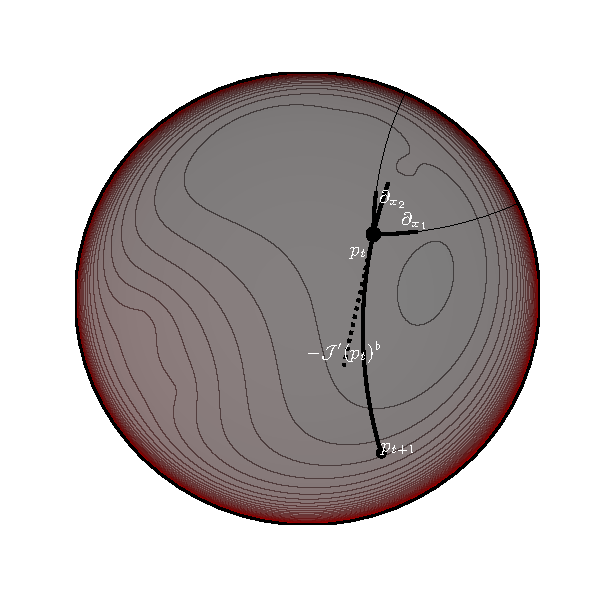
\includegraphics[width=.9\linewidth]{art/rgd-update.pdf}
\caption{A gradient descent step on the Poincar\'e disk.
Contour lines visualize the objective function; \( p_t \) is the current estimate;
    \( -\mathcal{J}'(p_t)^\flat \) is the descent direction, visualized as a geodesic curve;
\( p_{t+1} \) is the final point of that curve and the new estimate;
\( \partial_{x_1},~\partial_{x_2} \) are chart-induced basis vectors in the
    space of directions at \( p_t \);
stroked line visualizes the (downscaled) ``Euclidean'' gradient.
}
\label{fig:rgdStep}
\end{figure}

With all the tools introduced, we finally can describe the gradient descent
algorithm for an objective function \( J: M \to \mathbb{R} \) on an abstract
Riemannian manifold \( M \).
\begin{align*}
\dot x &= -\sharp(J'(x)),\\
x_{k+1} &\leftarrow \exp_{x_k}(-\eta \sharp(J'(x_k))).
\end{align*}

\subsection*{Higher-order methods}

Covariant derivative can be used to construct an analogue of Newton's
iteration. Of interest is also Betancourt's treatise on higher-order automatic
differentiation, based on jet theory~\cite{betancourt2018geometric}.

\section*{Retractions}

For many manifolds of interest we do \emph{not} know closed-form formulas for
exponential maps and parallel transport. Practical algorithms instead use their
approximations. A first-order approximation to exponential map is called
\emph{retraction} and there exists a large body of work on retraction-based
algorithms and their convergence, much of it associated with the name of
Pierre-Antoine Absil.

\section*{Trivializations}

Early works on hyperbolic neural networks (with parameters lying on manifolds)
mostly rely on Riemannian optimization. However, it has been empirically noted
for a long time that in experiments the naive tangent-space parameterization --
with parameters stored as coordinates of tangent vectors -- in conjunction with
standard adaptive gradient-based optimization algorithms in fact systematically
outperforms Riemannian optimization. This may be due to numerical instability
of the used models of hyperbolic space, or perhaps because coordinate-wise
adaptive methods like Adam play well in team with the very homogeneous and
symmetric hyperbolic space -- we do not know yet. However, alternatives have
been considered. Thus \citet{trivializations} does a good job at making sense,
mathematically, of optimization based on arbitrary parameterizations of a
surface by Euclidean vectors, with in-depth analysis of the three arguably most
important examples of such parameterizations: the Riemannian exponential map,
the Lie exponential, and retractions.

\section*{Gradient flow}

Because of apparent relation between differential equations and optimization
schemes, of interest also should
be~\citet{ambrosioGradientFlows,ambrosioOTSummerSchool}.

\section*{Barycentric subspace analysis}

\citet{baryPennec} discuss generalizations of Principal Component Analysis to
Riemannian manifolds and specifically discuss optimization on flags of linear
subspaces. This work is important to acquaint with at least because of a useful
language that it develops.
\section{Curvature} \label{sec:curvature}

\subsection*{Gromov hyperbolicity}

Early works on hyperbolic embeddings used to make vague claims about data
possessing ``hidden hyperbolic structure'' while avoiding exact definitions of
curvature, of which in fact there could be many. Later practitioners started
to refer to Gromov's~\cite{gromov} work introducing the \( \delta
\)-hyperbolicity. A \emph{pointed} metric space with distance \( d \) and reference point \( x_0 \) is called \( \delta \)-hyperbolic if
\[ p\cdot q \geq \min(p\cdot r, q\cdot r) - \delta, \]
for any points \( p, q, r \).
Here, for any \(x, y \) the \( x\cdot y \)
denotes the quantity \( \frac12 (d(x, x_0) + d(y, y_0) - d(x, y)) \).
It has also been acknowledged that this ``hidden curvature'' comes not from
just data, but from optimization problem: so the updated pre-print of
\citet{khrulkov} measures hyperbolicity of \texttt{MiniImageNet} by measuring
hyperbolicity of the distance between learned embeddings.

There's a more general framework of CAT (Cartan, Alexandrov, Toponogov) spaces
and \emph{curvature bounds} which I believe we (those interested in hyperbolic
deep learning) should master.

\subsection*{Synthetic: Curvature bounds}

\begin{figure}\centering
    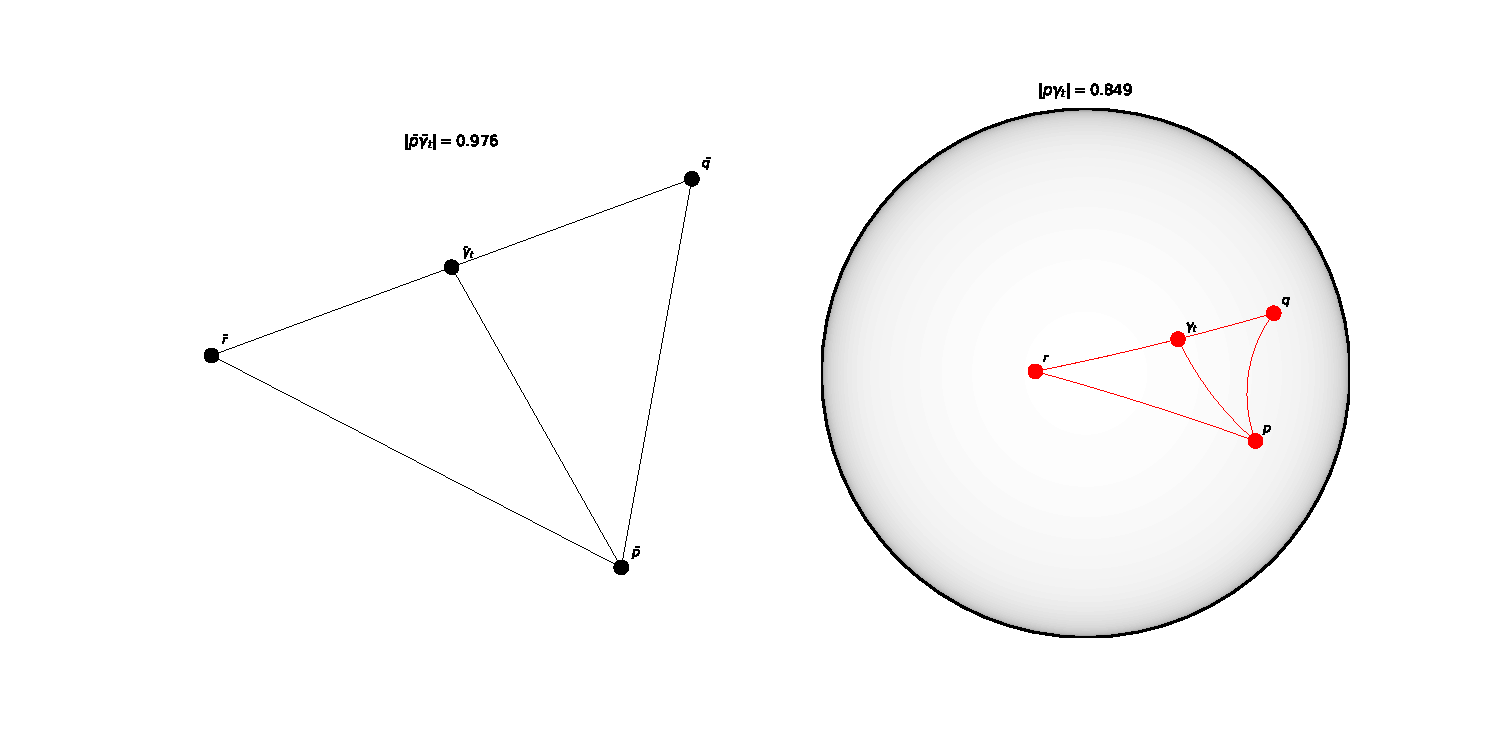
\includegraphics[width=.85\linewidth]{art/triangle-comparison.pdf}
    \caption{NPC Inequality: \( |\bar{p}\bar{\gamma}_t| > |p\gamma_t| \).
    Here
        \( M \) is a metric space;
        \( p, q, r \in M \) form a geodesic triangle;
        \( \bar{p}, \bar{q}, \bar{r} \in \mathbb{R}^2 \) is a Euclidean comparison triangle;
        \( \gamma_t \in M \) is a point on the constant-speed shortest path between \( q, r \);
        \( \bar{\gamma}_t \) is the corresponding comparison point.
    }
\end{figure}

Here should go an inspiring story about triangles and quadruples, but the time
doesn't allow us to include it.
For a motivating introduction, the Reader could refer to the most beautiful
talk of~\citet{villaniTriangles} and then his manuscript~\cite{villaniOldNew}.
\citet{burago} and \citet{alexander} give an introduction to metric geometry.
Less related are but inspiring are the seminal work of~\citet{sturm} on Wasserstein
distances between probability measures on metric spaces with curvature bounded
below, and~\citet{le2017existence}.

\subsection*{Analytic: Gauss, Riemann, Ricci}

Sectional and Gaussian curvature, come up as coefficients in the correction to
the the length of the hypothenuse of a triangle, and the area of a ball in a
curved space as compared to Euclidean prediction.
E.g. \citet{burago} describe Gaussian curvature in a (homogeneous and
symmetric) metric space as the number \( K(p) \) which appears in
\[ \operatorname{Vol}(B(p, r)) = \pi r^2 - \frac{\pi}{12}K(p) r^4 + o(r^4). \]

Ricci curvature is the quadratic form \( \operatorname{Ricci} \) that measures
the average of the sectional curvature \( \varkappa \):
\[ \operatorname{Ricci}(X) = \sum_{i=1}^n \varkappa(X, \partial_{x_i}). \]

Again, there isn't time and place to discuss this subject in depth, so the
Reader better refer to~\citet{leeRiem}.  Of interest also
are~\citet{feyCurv,gravityLight,burago}.

\section{Geoopt}

In the chapter~\nameref{chap:premises} we've discussed
~\nameref{sec:geoopt}~\cite{geoopt} we described our python package for
Riemannian optimization in PyTorch and perspectives for its further
development~\autoref{sec:geooptTodo}.
